\documentclass[12pt]{article}
\usepackage{parskip}
\usepackage{amsmath}
\usepackage{pdfpages}
\usepackage[margin=.6in]{geometry}

\begin{document}	

\includepdf[pages=12]{slides}
\includepdf[pages=13]{slides}
\includepdf[pages=14]{slides}
Evelutionary strategy is we are mutating our strategy as time goes on. Evolve our strategy, denoted $\sigma$, by varying how much exploration and exploitation you use. You add this to your current chromosomes, denoted X. Not all variables will see the same change. We add some learning/guidance to how we mutate our strategy to allow us to control how much we change each step. 

\includepdf[pages=15]{slides}
\includepdf[pages=16]{slides}
\includepdf[pages=17]{slides}
We assume that tau is the function of the size of the problem and all sigmas to be bounded.

\includepdf[pages=18]{slides}
Mutants have the same likilihood to be created, but some variable are more important than others so the data generated is not circular.

\includepdf[pages=19]{slides}
Here we have n variables that we are mutating. We create a correlation matrix to see how the variables effect each other. 

\includepdf[pages=20]{slides}
Here we have a normal distribution that is operating on a matrix and adding that to x. I think, fuck he explains nothing.

\includepdf[pages=21]{slides}
Here we things have tilted which means ... something.

\includepdf[pages=22]{slides}
We inherit from many parents. Basically just a much more complicated genetic algorithm. Not crossover, here we combine many parents into a single offspring.

\includepdf[pages=24]{slides}


\includepdf[pages=25]{slides}

\includepdf[pages=26]{slides}

\includepdf[pages=27]{slides}

\includepdf[pages=28]{slides}

\includepdf[pages=29]{slides}
We want to have some conditions for adaptation. These are some of them.

\includepdf[pages=34]{slides}
When we solve a problem we have a limited number of bits to do it, but we don't know the size of the problem. Since your program is evolving, the size of your solution must evolve as well. This rules out GA. For genetic programming our solution space will be graphs or trees. Here we are looking for function as solutions to problems, this is called calculus of variation. We dont necessarily mutate and crossover each time. Its more trigger based.

\includepdf[pages=35]{slides}
Here we are comnining trees into new subtrees that to randomly change (mutation). AS with before parent selection is based on fitness.

\includepdf[pages=36]{slides}
\includepdf[pages=37]{slides}
We are searching the space of formulas for one that optimizes some value. In this case we want to look at the number of children and income when giving way loans to maximize the amount of money the bank makes. 

\includepdf[pages=38]{slides}
So here is how we represent the solution as a tree. We can have many different trees from this to evaluate.

\includepdf[pages=43]{slides}
\includepdf[pages=44]{slides}
\includepdf[pages=45]{slides}
\includepdf[pages=47]{slides}
This is a comparison of GA and GP. At every step we debate about whether you want to mutate or crossover.

\includepdf[pages=48]{slides}
Terminals are values (operands) and functions that you apply to them. Think way back go compliers with syntax trees.
 
\includepdf[pages=50]{slides}
\includepdf[pages=51]{slides}
Here we randomly generated the tree and mutated it by picking a node an add a subtree to it.

\includepdf[pages=52]{slides}
We want the probability of mutation to be rather small. Remember that children can be bigger than their parents.

\includepdf[pages=53]{slides}
\includepdf[pages=54]{slides}
As with always we chose parents based on fitness. 

\includepdf[pages=55]{slides}
Start the tree at some maximum depth you populate the terminals (they don't have to all be on the same level).

\includepdf[pages=56]{slides}
We might accidentally become too interested in one branch where we keep adding to it so it gets  massive. 

\includepdf[pages=57-83]{slides}

Soooo, he jumped to another slide set that I can't find. Weeeeeeee. Mother fucker

\textbf{Sufficiency}: a solution to the problem at hand must exist in the space of prgams created from the fuction set and the terminal set

\textbf{Closure}: every function must be campable of accepting the values of every terminal from the terminal set and every function from the function set

One way to get around closure is to make all terminals and functions return the same type or use strongly typed genetic programming to ensure that all expressions are type safe.











\end{document}